\chapter{Quality-Aware Load-Shedding}
\label{ch:load_shedding}

This chapter describes the overload management techniques employed by the \sys
system. In particular, it focuses on the \emph{load-shedder} component and explains how it uses the \sic
values to make semantic load-shedding decisions about which tuples to discard. 
The goal of the \mbox{load-shedding} mechanism is to manage overload by discarding a portion of the input
tuples. The algorithm that decides which tuples to keep and which to shed leverages the information
contained in the \sic values of tuples to implement an intelligent and fair load-shedding policy.

% The description of the shedding module follows an abstract model formed by three components. When tuples
% are received by a node, they are stored in an input buffer waiting to be processed. If the size
% of this buffer grows out of control, the system becomes overloaded. The \emph{overload detector} is in
% charge of monitoring the performance of processing nodes, it identifies overload conditions and trigger
% the \emph{tuple shedder} to discard tuples.
Using the \sic values, it is possible to implement a \emph{fair shedding} policy that attempts to
penalise all queries in a similar fashion. In this context, we define fairness based on
processing quality (\ie a system is fair if all queries achieve the same \sic values for their results).
Before introducing the load-shedding algorithm, the main components of the overload management
infrastructure are presented.

As part of the load-shedding process, the system first has to choose how many tuples to keep for
processing.
This estimate is made using a simple \emph{cost model}, which takes into account the average time spent
processing a generic tuple. 
Next, a choice has to be made about which tuples to keep.
A fair shedding algorithm is presented in Section~\ref{sec:fair-shedding}, which uses the \sic
values of the incoming tuples to select the set of tuples to be discarded so that all queries experience
the same reduction in the quality of their processing.

\mbox{Load-shedding} is carried out in a system that is already overloaded so that it can keep on
processing even after some of the input was discarded. In a scenario in which the processing node runs
out of CPU cycles, the overload management infrastructure has to calculate the correct set of tuples to discard according to a given shedding policy. 
The chapter finishes with a description of the details of the \mbox{load-shedding} mechanisms
employed by the DISSP system.

%\clearpage
%--------------------------------------------------------------------------------------------------------

\section{Fairness in \mbox{Load-Shedding}}
\label{sec:fls}

A processing node is considered overloaded when it cannot process all the data that it receives as input
in a timely fashion. If, in a given time interval, the amount of incoming tuples (\ie the \emph{input
rate}) is larger than the number of tuples that the system can process (\ie the \emph{output rate}) the
processing capacity of that node is exceeded. When this occurs, the internal queues of pending tuples
increase in size. While such a condition can be sustained for a short amount of time, it leads eventually
to an exhaustion of memory if it is not addressed.
An overload condition can be caused by an increase in the rate of incoming tuples or
by a change in the processing cost of tuples.

Augmenting streams with \sic values allows the system to reason about the quality of tuples. Our quality
metric is designed to capture the amount of information lost during the creation of a tuple, and thus its
contribution to the query results.
% Employing the information carried by the \sic metadata allows the system to reason about the quality of
% the data it processes. 
As a result, the system can predict the impact of discarding a given tuple on the quality of the final
results of a query. This allows for the implementation of an \emph{intelligent shedding policy}.
Section~\ref{sec:fair-shedding} explains the details of such a \emph{fair shedding policy}, which
attempts to equalise the resulting \sic values of all queries.

In a shared infrastructure, the available processing resources are divided among potentially a large
number of concurrently running queries. In this context, a \emph{fair} system would allocate a proportional amount
of resources to each query so that, in an overload condition, the quality degradation of results is
similar across all queries. Employing the \sic metric to quantify the reduction in information content
in the results allows for a more precise definition of fairness in a stream processing system.
\begin{definition}[Fairness in a Stream Processing System]{
An overloaded stream processing system that performs load-shedding is considered to be fair if it
discards tuples in a way that minimises the difference in the \sic values of results for all running
queries.
}
\end{definition}	
This definition does not depend on the amount of resources consumed by a query or on
the number of operators that it contains. Each query is treated equally and allocated an amount of
resources that is proportional to its needs. This means that each query should achieve the same
\mbox{quality of processing}. A policy that allocates the same amount of resources to all queries
would favour small queries, while expensive queries would be penalised. This would lead to a large spread
between the \sic values of the light and the heavy queries. The goal of a fair system, according to
the above definition, is instead to equalise the \sic values of all queries, trying to reduce the differences
among queries as much as possible.

%--------------------------------------------------------------------------------------------------------
   
\section{Abstract Shedder Model}
\label{sec:abs-shedder}

Figure~\ref{fig:ls_model} shows the \emph{abstract model} of a load-shedder. It depicts the three generic
components that are needed to implement an overload management mechanism. When tuples are
received, they are staged in an \emph{input buffer}, waiting to be processed. Periodically, the \emph{overload detector}
checks if the load of the system is acceptable or if some of the input has to be discarded. In case the
node is considered to be overloaded, it executes the \emph{tuple shedder}, which selects and discards a
certain number of tuples in order to overcome the overload situation.
 
\begin{figure}[b]
	\centering
	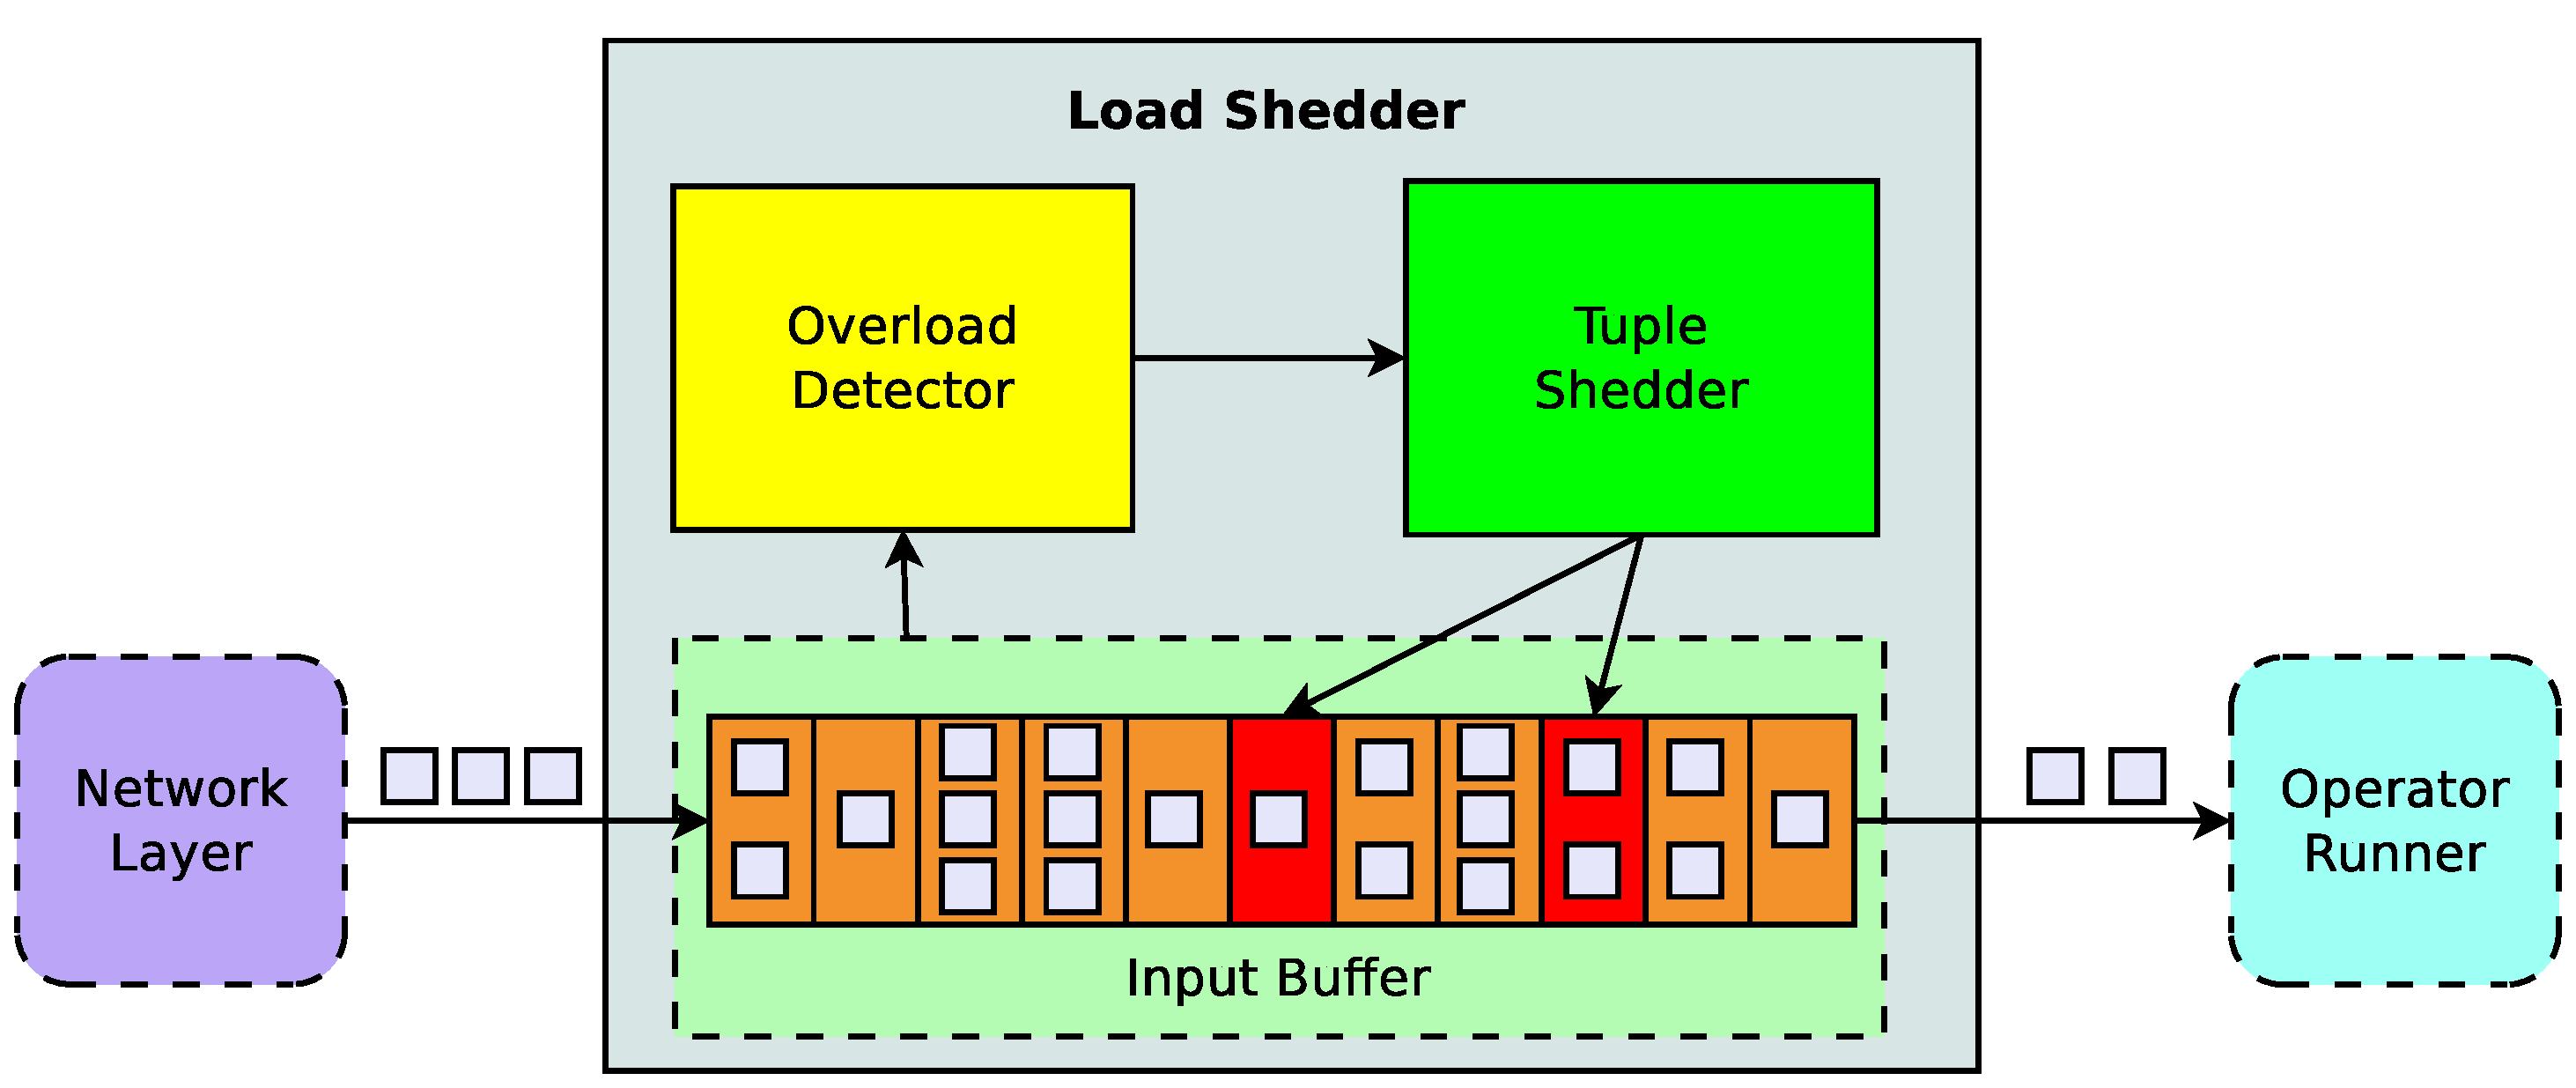
\includegraphics[width=0.9\textwidth]{img/tesi/ls_model} 
	\caption{Abstract representation of a load-shedder, showing its internal conceptual model.}
	\label{fig:ls_model}
\end{figure}   

\subsection*{Input Buffer} 

The tuples that are received by a node are stored in an input buffer waiting to be
processed.
This allows the system to continue receiving tuples from the network, even though it is unable to consume
them at the same rate.
The order in which tuples are stored follows the FIFO model, thus preserving the natural temporal
order of tuples. Every time a processing thread becomes available, it removes the oldest tuple from the
input buffer and proceeds with its processing. 

When the system is overloaded, the size of the input buffer grows, as more tuples are admitted than
processed. This leads to an increase in the latency of results and eventually to the exhaustion of system resources.
If the size of the input buffer starts to grow, the overload detector invokes the
tuple shedder to control its size.\\
An input buffer also allows the system to implement a \emph{semantic shedding policy}.
Instead of discarding tuples as they arrive, the system stores them first in the
input buffer and leaves the decision about which tuples to discard to the tuple shedder. This component
implements the shedding algorithm that chooses which tuples to discard among those
awaiting processing in the input buffer.

\subsection*{Overload Detector} 

The overload detector is responsible for monitoring the load of a processing node. It detects an
overload condition before it becomes critical and invokes the tuple shedder to discard a fraction of the
input in order to contain the load within the operational limits of the node.
Periodically, at fixed \emph{shedding intervals}~$\delta$, the overload detector checks the size of the
input buffer.
The shedding interval is set as a system parameter and influences the behaviour of the system. 
For low latency processing, it is preferable to set this to a short time interval, in the order of a few
hundreds of milliseconds (\eg 250ms). On the other hand, setting the value too low induces unnecessary
overhead due to frequent shedder invocations.

After each shedding interval, the overload detector makes a prediction about the number of tuples that
the system is able to process during the next interval, which is referred to as $N_{keep}$. In order
to estimate this amount correctly, the overload detector uses a \emph{tuple cost model}, as
described in Section~\ref{sec:arch-cost_model}. 
The difference between the total number of tuples in the input buffer, $\textit{IB}_{size}$, and the
predicted throughput of the system in the next shedding interval, $N_{keep}$, is the number of tuples
to be discarded by the tuple shedder, $N_{discard}$.
\begin{align}
	N_{discard} = \textit{IB}_{size} - N_{keep}
\end{align}
If $N_{discard}$ is negative, there is no need for shedding during this interval. If its value is
positive, the tuple shedder is invoked. According to a shedding policy, the tuple shedder then calculates
which tuples to discard among those available in the input buffer.

\subsection*{Tuple Shedder} 
\label{sec:arch-tuple_shedder}

After the overload detector identified an overload condition, it invokes the tuple shedder to discard
a certain number of tuples from those awaiting processing in the input buffer.
The number of tuples to be shed is calculated by the overload detector but the choice of which tuples
to discard is made by the tuple shedder. 
It inspects the input tuples and selects the ones to shed based on a \emph{shedding policy}.

To better understand the interactions among the different components of this abstract shedding model, let
us consider again Figure~\ref{fig:ls_model}. Tuples are received by the \emph{network layer} and are
placed into the \emph{input buffer} even if the node is currently overloaded because \mbox{load-shedding}
decisions are made later. Each tuple received by a node awaits processing in the input buffer until it
gets either selected for processing and passed to the \emph{operator runner}, or discarded by the
\emph{tuple shedder}. The \emph{overload detector} decides if the amount of tuples
currently in the input buffer can be managed by the operator runner or if instead some tuples should
be discarded to avoid overload. When the overload detector estimates that $N_{keep}$ tuples should be
discarded, it invokes the tuple shedder passing $N_{keep}$ as a parameter. At this point, the tuple
shedder chooses $N_{keep}$ tuples among those currently available to be saved.
This decision is made based on a \emph{\mbox{load-shedding} policy}, which is implemented within the tuple
shedder. The simplest policy is a \emph{random} one, in which tuples are discarded arbitrarily.

Augmenting tuples with the \sic quality metric enables the tuple shedder to
implement a more intelligent shedding policy that takes into account the amount of information captured
by each tuple.
The use of metadata information about the quality of tuples permits the implementation of a
\emph{semantic shedding} algorithm, which can be used to maintain certain properties among queries. The
next section describes the design of a \emph{fair shedding} algorithm, which aims at penalising all
queries in a similar fashion.
%--------------------------------------------------------------------------------------------------------

\section{Quality-Aware Fair Shedding}
\label{sec:fair-shedding}

% This section describes the implementation of the fair shedding algorithm
% (Algorithm~\ref{alg:distributedFairness}) employed by every \sys node. 
This section describes the implementation of a \emph{fair shedding} policy, following the principles
stated in Section~\ref{sec:fls}. The goal of this policy is to achieve a fair resource
allocation for all queries running into the system. The policy strives to equalise the \sic values
achieved by the result tuples of all queries.  
The tuple shedder selects the tuples to be discarded, trying to equalise the processing
degradation of all queries so that their normalised (\ie in the [0,1] interval) result \sic values
are numerically close.
The tuple shedder addresses overload conditions by periodically discarding batches, enabling the node
to retain a sustainable throughput of processed tuples with low queueing delays. 

When the shedder is invoked by the \emph{overload detector}, it selects
$N_{keep}$ tuples to keep from the its input buffer queue.  At first, the shedder
assumes that all batches must be discarded. Next, it gradually admits batches
that belong to queries that would otherwise suffer from the largest
reduction in their \sic values. This process terminates when the shedder has
admitted the required number of tuples as determined by the overload detector.
During the shedding process, the shedder always considers the normalised
\sic values of the tuples for comparisons among queries. 

Next, we present a \emph{tuple cost model} to estimate the
processing capacity of a node. The cost model is used by the overload detector to calculate if the node
is overloaded and to predict the number of
tuples that the system can process before the next shedding interval.
We also present a description as pseudocode of the algorithm realising the
fair shedding policy, providing a detailed explanation of the involved steps.

% \paragraph*{Multi-fragment queries}
% 
% %When queries are decomposed into multiple fragments across nodes, the tuple
% %shedder is aware only of the tuple processing at its local node. Since shedding
% %happens at other nodes as well, the tuple shedder must receive the remote
% %result \sic value of a multi-fragment query. This is done by the query
% %coordinator, which periodically (\eg every 1~sec) submits the result \sic value
% %to all nodes that participate in the execution of a query. 
% 
% %This input is used by the tuple shedder, as follows. Let's assume that a query is
% %deployed across two nodes and each query fragment processes tuples from half of
% %the sources. In this case, the total possible \sic contribution of tuples from
% %each node to the result \sic is 0.5. If the node also executes another query
% %fragment, each would receive the same rate of tuples per second. The shedder
% %now has to rank these two queries to find the most penalised in terms of result
% %\sic values when all tuples are discarded. By only considering the loss in the
% %IB, the shedder would estimate that the two queries suffer equally. In reality,
% %discarding a tuple from each query has a different effect on their \sic values
% %depending on whether other nodes discard tuples of a multi-part query.
% 
% To consider query partitioning in shedding decisions, the shedder calculates
% the projected result \sic, $\hat{q}_{SIC}$, as the difference between the result \sic value
% of the query and the total \sic contributions of batches predicated to be
% discarded from the IB queue, as shown in line~$9$ of Algorithm~\ref{alg:distributedFairness}.
% 
% \paragraph*{Differences in inter-arrival rates}
% 
% %In general, the processing of the low-rate queries is more penalised than that
% %of high-rate queries. For example, consider two queries with one query fragment
% %overloading the same node. One query receives $x$~batches for each shedding
% %interval, whereas the other query only receives $x$~batches every few
% %intervals. When the IB contains batches from both queries, the shedder is
% %likely to discard batches from both queries. Therefore, low-rate query suffers
% %more in terms of a reduction of its \sic values.
% 
% To address different arrival rates of tuples in streams, the shedder must
% maintain a history of the \sic values of tuples admitted by each query. It
% records a summary of tuples admitted for each query and also for each stream
% within a query. The shedder then uses this information when selecting the
% tuples to admit.
% 
% % To counteract this effect, the shedder must maintain a history of the tuples
% % admitted for each query.

\subsection*{Tuple Cost Model}
\label{sec:arch-cost_model}

A processing node is overloaded when the aggregate resource demand for executing hosted operators of
queries exceeds the resource capacity of the node. 
% In particular, every \sys node maintains an \emph{input buffer}~(IB) queue, in which all incoming tuples
% from other nodes or sources await processing.
When the rate of tuple arrival exceeds the processing capacity of the node, the size of the input buffer
grows and the node becomes overloaded.

To calculate the number of tuples to admit for processing, a node has to estimate the processing cost of
tuples when executing different types of operators and queries. We employ a simple cost model to
calculate the \emph{average} processing time spent on a given tuple for a query. We then use the past
resource consumption when processing tuples to estimate future resource demands.
We assume that the average tuple processing cost~$C_T$ is:
\begin{align}
C_T = t / n
\end{align} 
where $t$ is the time interval elapsed between invocations of the overload detector and $n$ is the
number of tuples processed by that node during $t$. $C_T$ is the time that the node spent on average
processing a tuple from a query.
For an accurate estimation of $C_T$, we use the measured time interval~$t$,
instead of the fixed interval~$\delta$, which is the theoretical time interval between executions of the 
overload detector.
In a real system, the measured time~$t$ between successive invocations of the overload detector
may differ from $\delta$. To compensate for any such differences and to have an accurate
estimation of $C_T$, we use the measured elapsed time $t$ rather than the fixed
interval $\delta$. 

Thus, the estimated number of tuples that the system is able to process between successive invocations
of the overload detector is:
\begin{align}
N_{keep} = \delta / C_T
\end{align} 
where $\delta$ is the fixed time interval between shedding invocations, and $C_T$ is the average time
spent processing a tuple.
To estimate the value of $N_{keep}$, we use a sliding window to avoid transient rate
fluctuations that would lead to under- or over-prediction of the true number of tuples that a node can
process. Employing a sliding window allows for a smoother estimate, which is more resilient to sudden
changes of the incoming tuple rate.

\begin{figure}  
	\centering
	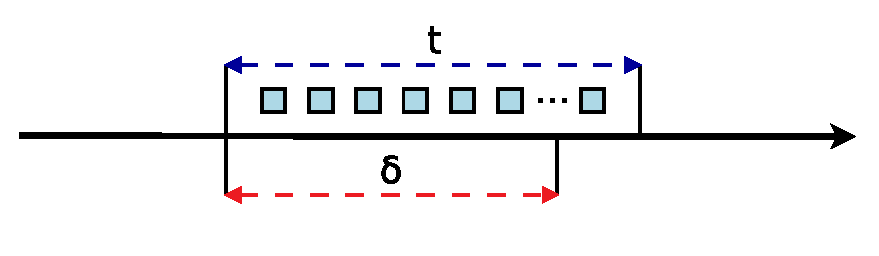
\includegraphics[width=0.7\textwidth]{img/tesi/tuple_cost} 
	\caption{Graphical representation of the time intervals $\delta$ and $t$ used to calculate the
	\emph{average tuple cost} $C_T$ needed to predict the \emph{future processing capacity}
	$N_{keep}$ of a node.}
	\label{fig:tuple_cost}
\end{figure} 

Figure~\ref{fig:tuple_cost} shows the two time intervals, $\delta$ and $t$ used to calculate the cost of
a tuple and the average time needed to process an arbitrary tuple, respectively. Let us assume a shedding
interval $\delta$ of 250 milliseconds. In practice, the \emph{overload detector} triggers with a small
delay, \eg after a time $t$ of 300 milliseconds. During this time, the system processes 5000 tuples.
Therefore, every tuple has a cost $C_T$ of $0.06$~ms/tuple. The system thus predicts that in the next $\delta$ interval it will
have the processing capacity $N_{keep}$ of approximately  $4100$ tuples. This value is
smoothed by a sliding average.

More complex cost models were proposed in the past~\cite{expensivepredicatejoin07,
evaluatingwindow03}. These approaches are tailored for certain types of operators, such as joins, and
require the tuning of a number of parameters for accurate estimation. Instead, we strive for a general
cost model that can be applied to any type of query or operator. Our approach assumes that the cost of processing a tuple
remains fairly constant and is similar across operators. This is not always true, though, as some
operators may require significantly more time to process tuples depending on their contents. A
more precise cost model would also take the semantics of the query into account, \eg considering the
types of operators. 
% For the scope of this work, a simpler cost model has been preferred.

\subsection*{Quality-Aware Fair Shedding Algorithm}
\label{sec:fairness-algo}

The algorithm used by the tuple shedder to implement the fair shedding policy is specified using the
pseudocode in Algorithm~\ref{alg:distributedFairness}. The main idea behind it is to start by considering
all tuples as discarded. Next, it estimates the reduction in \sic values experienced by each query,
making a ranking. It iterates, adding one batch of tuples at the time, and chooses the one with the
highest \sic contribution from the query with the lowest estimated \sic value. After each step, it
recalculates the ranking and it retains tuples until it reaches the limit given by the overload
detector. The rest of this section provides a more detailed description of the algorithm.

First, the input buffer queue is locked by the tuple shedder~(line~$1$). This means that the system stops
accepting new incoming batches and current batches in the queue are not processed by operators. While the
shedder runs, new incoming batches are held temporarily in a secondary buffer, which is merged with the
input buffer queue before the node resumes processing. This allows the \emph{tuple shedder} to consider a
snapshot of the current situation so that it reasons based on a static set of pending tuples.

The \emph{tuple shedder} then considers all batches in the input buffer as discarded~(lines~$2$--$8$). 
This algorithm works at the granularity of \emph{batches} not tuples, which reduces the number of
iterations and thus the associated overhead.

\begin{algorithm}[b!] 
  \SetKwInOut{Input}{Input}\SetKwInOut{Output}{Output}
  \Input{number of tuples to save ($N_{keep}$), input buffer (IB)\\}
  \Output{input buffer (IB) containing $N_{keep}$ tuples, or less if not enough}

        lock IB\\
	\ForEach{query $\in$ node}
	{
		update $Q_{SIC}$ of $query$
	}
        \ForEach{batch $\in$ IB}
        {
		find query $Q$ such that $batch \in Q$ \\
		update ${Q}_{SIC}$ as if $batch$ was discarded \\
  		move $batch$ to priority queue of queries (increasing ${Q}_{SIC}$) and for each query keep batches in
  		descending \sic order\\
		remove $batch$ from IB\\
        }
	$n_{\mathrm{tuples}}^{\prime} = 0$\\
        \While{ $N_{keep}^{\prime} < N_{keep}$ } {
                Q := pick query with the least ${Q}_{SIC}$ \\
                b := pick batch from Q with highest \sic \\
        	add b to IB\\
		update ordered list of queries\\
		Add tuples in b to $N_{keep}^{\prime}$ \\
        }
        unlock IB\\
\caption{Tuple shedding with SIC fairness}
\label{alg:distributedFairness}
\end{algorithm}

First, it updates the current result \sic values of all queries~(lines~$2$--$3$). 
For each query that has batches in the input buffer queue, the tuple shedder calculates the new projected
\sic value as if none of its batches would be processed~(line~$6$).
After that, it adds all active queries (\ie ones that have at least one pending batch) to a priority
queue sorted by increasing projected \sic values. In this way, it can quickly identify the query with
the lowest projected performance so that a batch from it can be retained.

Next, the shedder removes all batches in the input buffer. It moves them to a temporary 
buffer and groups them according to the query that they belong to, while keeping an ordered list of
queries and batches for each query~(line~$7$).
One by one, all batches are moved from the input buffer and inserted into a set of priority
queues, one for each query. This builds an ordered list of batches for each query, sorted by decreasing
\sic values. Once the tuple shedder decides to save one more batch of a certain
query, it can quickly select the one with the highest \sic value, and thus the most valuable one, by
simply removing the head of a priority queue.

All batches are gradually removed from the input buffer~(line~$8$). 
This ensures that the shedder has to parse all batches in the input buffer only once 
and simultaneously builds the required priority queues for the next part of the shedding decision. 
A priority queue of queries is also created, ordered by increasing \sic values, so that the head of the
queue is always the query with the worst projected \sic value~(line~$7$).

Next, the shedder considers which tuples to admit from each query to achieve fairness~lines~($10$--$15$). 
It first selects the query that would be penalised the most (\ie the one with the
lowest projected \sic value)~(line~$11$). It then selects the
batch with the highest \sic value for this query~(line~$12$).
By selecting the batch with the highest \sic value among those available for each query, the
system maximises the projected \sic value, adding first the batches with the greatest contribution.

The shedder moves the selected batch back to the input buffer for processing~(line~$13$). 
Since the batch is not discarded, the shedder also updates the projected \sic value of the query
whose batch was saved and the priority queue of queries~(line~$14$).
The shedder repeats this process until it has accepted $N_{keep}$~tuples.
Any remaining batches from the temporary buffer are discarded and regular tuple processing
from the input buffer queue resumes~(line~$16$). 
 
% \subsubsection*{Algorithmic Complexity}
% 
% %The algorithm makes a number of passes over the input buffer, 
% 
% %First, it has to update the \sic values of each query, thus using an amount of time proportional to the
% %number of queries $O(N_q)$ having a subquery running at this node. 
% %\mnote{Not quite sure actually, it would be interesting to go over it together.}
% \todo

%\clearpage

%----------------------------------------------------------------------%
\section{Implementation of the DISSP Load-Shedder}

This section provides implementation details about the overload management system that is part
of the \sys prototype system. It describes how the abstract components are realised
in practice and outlines some of the mechanisms that have been employed to achieve robustness under
overload.

\textbf{Input Buffer.} The input buffer is the internal pending jobs queue of the ThreadPoolExecutor, the
pool of processing threads implementing the \emph{operator runner}. It contains a series of WorkUnits
objects that each bundle a batch of tuples and a reference to their destination operators and represent
future processing units. When the overload detector identifies a critical load situation, it
calculates the maximum length of the input buffer and triggers the tuple shedder to remove the
excess tuples from the input buffer.

\textbf{Overload Detector.} The overload detector is implemented by the CheckOverload class, which
realises a monitoring thread that performs a check on the current system load at each shedding
interval. This thread maintains certain statistics about the performance of the system and acts if it
detects an overload condition. It calculates the average \emph{tuple cost}  (\ie the time needed to
process one tuple using the cost model previously explained). Based on this tuple cost, it makes a
prediction about the number of tuples that the system will be able to process during the next shedding
interval, thus inferring the maximum number of tuples that should be present in the input buffer. If
there are currently more tuples awaiting to be processed in the queue, it invokes the tuple shedder that
chooses which tuples should be discarded in order to maintain a sustainable system load.

\textbf{Tuple Shedder.} The tuple shedder is the class implementing the \mbox{load-shedding} semantics.
It contains the algorithm that chooses which tuples to discard from the ones currently awaiting
processing in the input buffer. It exposes a simple interface to the overload detector, which
includes a parameter with the number of tuples to keep in the buffer.
The internal shedding policy analyses the input buffer queue and decides which tuples to discard.
By hanging the class implementing the tuple shedder interface, it is possible
to realise different shedding policies. In its simplest implementation, it discards tuples at
random. However, by exploiting the \sic quality metric, it is possible to implement a semantic
approach, such as the fair shedding algorithm presented in this chapter.

\textbf{Late Deserialisation.} When tuples are received by the network layer, they are placed
directly into the input buffer waiting for processing. At this point, the data remain in
network representation and needs to be converted first into concrete objects before it can be processed.
This \emph{deserialisation} step of the input tuples is costly and, therefore, delayed as much as
possible in order to avoid spending CPU cycles on tuples that may never be processed. The system
deserialises only the minimum required information, such as the query id to which the tuples belong
and their \sic value. Using this information, the tuple shedder executes its shedding policy and decides
if a batch of tuples is valuable enough to be preserved. The final
deserialisation happens only when the WorkUnit is selected for processing. It is the first step performed
by the operator runner when it removes the WorkUnit from the input buffer.

\textbf{Sliding Windows.} The load experienced by a stream processing node can vary dramatically over
time. As a consequence, when considering a few hundred milliseconds, the number of
tuples delivered to the node can be highly variable. It is important that the overload detector does
not mistake the arrival of an isolated large batch of tuples, which can be safely kept in the input
buffer, with the beginning of a long term overload condition. For this reason, when
implementing the tuple cost model, the system uses a moving average
calculated over the last $N$ values of the metric. This adds slack in the reaction
of the system and allows it to distinguish between a sudden load spike, which can be ignored, and
a sustained change in the load, which must be addressed.

%----------------------------------------------------------------------
\section{Summary}

This chapter presented a quality-aware load-shedder component of a stream processing system, which
detects and addresses the excess of processing load by discarding a portion of the input tuples. In
particular, the chapter proposed to exploit the \sic quality metric to implement an intelligent shedding
policy, which tries to allocate resources fairly among queries. First, we defined \emph{fairness} in a
stream processing system based on the \sic values achieved by queries. We then described an abstract
model for the overload management system, explaining the interaction among its internal components. 
Based on this, we presented an algorithm that implements a \emph{fair shedding policy} used to
equalise the achieved \sic values of all queries. We showed how a tuple cost model is required to
estimate a sustainable throughput and thus the number of tuples to be shed, and how to choose which
tuples should be discarded using the \sic metric. The chapter ended with a description of implementation
details of such component in the \sys prototype system. 



